\subsection{ทดสอบประสิทธิภาพการทำงานของโมเดลปัญญาประดิษฐ์สำหรับการระบุตัวตนของบุคคล}
\label{sec:reid_ex}
ความแม่นยำของโมเดลปัญญาประดิษฐ์จากแหล่งที่มีมามีค่าดังตารางด้านล่างดังนี้
\begin{table}[!ht]
    \centering
    \begin{tabular}{|c|c|}
            \hline
            {โมเดลปัญญาประดิษฐ์}&{rank1/mAP โดยใช้วิธีการทดสอบด้วย Global+DMLI}				\\
            \hline
            ResNet50 Market1501	 			& 91.0/77.6								\\
            ResNet50 DukeMTMCReID			& 80.7/68.0								\\
            ResNet50 CUHK03				& 60.9/59.7								\\
            ResNet50 MSMT17				& 66.3/40.6								\\
        \hline
    \end{tabular}
    \caption{ผลการทดสอบความแม่นยำของโมเดลปัญญาประดิษฐ์}
    \label{tab: Accuracy of model ReID}
\end{table}
\\
ต่อมานำโมเดลปัญญาประดิษฐ์แต่ละอันมาทดสอบกับตัวอย่างภาพชุดข้อมูลที่ทางคณะผู้วิจัยได้สร้างขึ้น โดยภาพชุดข้อมูลที่นำมาใช้จะผ่านการตรวจหาบุคคลภายในภาพด้วยโมเดลปัญญาประดิษฐ์ YOLO-v3 spp นำภาพชุดข้อมูลที่ผ่านการตรวจหาบุคคลภายในภาพเข้าระบบการระบุตัวตนของบุคคล โดยจะให้ผลลัพธ์ออกมาเป็นค่า AUC และกราฟที่แสดงการเปรียบเทียบระหว่างการระบุว่าเป็นบุคคลเดียวกันไม่เป็นบุคคลเดียวกันตามรูปที่ \ref{fig: กราฟแสดงการเปรียบระหว่างการระบุว่าเป็นบุคคลเดียวกันกับไม่เป็นบุคคลเดียวกัน}

\begin{figure}[!ht]
    \centering
    \begin{subfigure}[b]{0.4\textwidth}
        \centering
        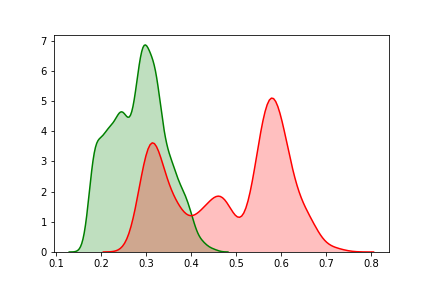
\includegraphics[width=\textwidth]{chapter4/images/graph_market.png}
	\caption{กราฟของโมเดลปัญญาประดิษฐ์ที่ผ่านการสร้างด้วยชุดข้อมูล Market1501}
        \label{fig:graph_market}
    \end{subfigure}
    \hfill
    \begin{subfigure}[b]{0.4\textwidth}
        \centering
        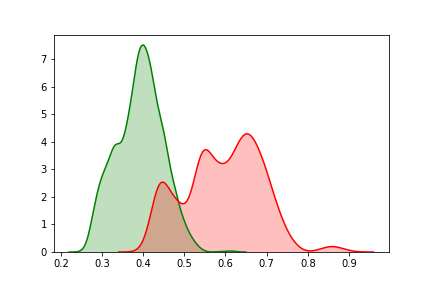
\includegraphics[width=\textwidth]{chapter4/images/graph_dukemtmc.png}
	\caption{กราฟของโมเดลปัญญาประดิษฐ์ที่ผ่านการสร้างด้วยชุดข้อมูล DukeMTMCReID}
        \label{fig:graph_dukemtmc}
    \end{subfigure}
    \hfill
    \begin{subfigure}[b]{0.4\textwidth}
        \centering
        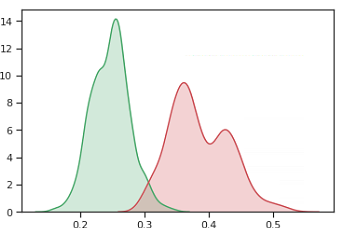
\includegraphics[width=\textwidth]{chapter4/images/graph_cuhk.png}
	\caption{กราฟของโมเดลปัญญาประดิษฐ์ที่ผ่านการสร้างด้วยชุดข้อมูล CUHK03}
        \label{fig:graph_cuhk}
    \end{subfigure}
    \hfill
    \begin{subfigure}[b]{0.4\textwidth}
        \centering
        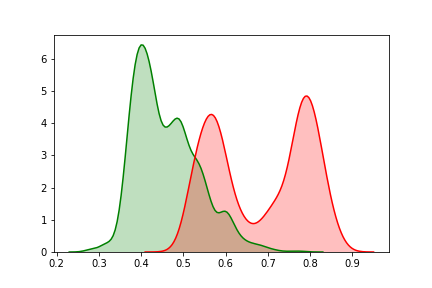
\includegraphics[width=\textwidth]{chapter4/images/graph_msmt.png}
	\caption{กราฟของโมเดลปัญญาประดิษฐ์ที่ผ่านการสร้างด้วยชุดข้อมูล MSMT17}
        \label{fig:graph_msmt}
    \end{subfigure}
    \hfill
    \caption{กราฟแสดงการเปรียบระหว่างการระบุว่าเป็นบุคคลเดียวกันกับไม่เป็นบุคคลเดียวกัน โดยพื้นที่ใต้กราฟที่เป็นสีเขียวจะหมายถึงการระบุว่าเป็นบุคคลเดียวกัน ในขณะที่พื้นที่ใต้กราฟสีแดงหมายถึงการระบุว่าไม่เป็นบุคคลเดียวกัน และแกน x คือค่า aligned distace ส่วนของแกน y จำนวนคู่ของภาพ  }
    \label{fig: กราฟแสดงการเปรียบระหว่างการระบุว่าเป็นบุคคลเดียวกันกับไม่เป็นบุคคลเดียวกัน}
\end{figure}
\clearpage
\begin{table}[!ht]
    \centering
    \begin{tabular}{|c|c|}
            \hline
            {โมเดลปัญญาประดิษฐ์}&{AUC}											\\
            \hline
            ResNet50 Market1501	 		& 0.94								\\
            ResNet50 DukeMTMCReID		& 0.94								\\
            ResNet50 CUHK03				& 0.99								\\
            ResNet50 MSMT17				& 0.86								\\
        \hline
    \end{tabular}
    \caption{ผลการทดสอบค่า AUC ของโมเดลปัญญาประดิษฐ์}
    \label{tab: AUC of model ReID}
\end{table}

จากการทดลองสมมติฐานที่ตั้งไว้นั้นไม่เป็นจริง เพราะโมเดลปัญญาประดิษฐ์ที่ผ่านการสร้างด้วยชุดข้อมูล Market1501 นั้นไม่ได้มีค่า AUC สูงที่สุดเมื่อนำมาใช้กับชุดข้อมูลที่ทางผู้วิจัยสร้างขึ้น เมื่อเทียบ โมเดลปัญญาประดิษฐ์ที่ผ่านการสร้างด้วยชุดข้อมูล CUHK03 นั้นที่ให้ผลลัพธ์ค่า AUC สูงที่สุดเมื่อนำมาใช้กับชุดข้อมูลที่ทางผู้วิจัยสร้างขึ้น ทางผู้วิจัยจึงได้เลือกโมเดลปัญญาประดิษฐ์ที่ผ่านการสร้างด้วยชุดข้อมูล CUHK03 นี้มาใช่ในงานวิจัย